\documentclass [xcolor=svgnames, t] {beamer}
\usepackage[utf8]{inputenc}
\usepackage{booktabs, comment}
\usepackage[absolute, overlay]{textpos}
\usepackage{pgfpages}
\usepackage[font=footnotesize]{caption}
\useoutertheme{infolines}

\setbeamertemplate{page number in head/foot}{}
\usepackage{csquotes}


\usepackage{amsmath}
\usepackage[makeroom]{cancel}


\usepackage{textpos}

\usepackage{tikz}

\usetheme{Madrid}
\usepackage{tikz}



\title[Chatterjee's Correlation in MCMC]{Applications of Chatterjee's Correlation in MCMC}
\subtitle{(UGP, 21-22 Even Semester)}
\institute[IITK]{Department of Mathematics and Statistics \\Indian Institute of Technology, Kanpur}
\titlegraphic{
\includegraphics[height=2.0cm]{iitk_logo.jpg}}
\author[Vivek Kumar Singh]{
	Vivek Kumar Singh,
	Dootika Vats }


\institute[]{Department of Mathematics and Statistics \\Indian Institute of Technology, Kanpur}
\date{\today}


\addtobeamertemplate{navigation symbols}{}{%
    \usebeamerfont{footline}%
    \usebeamercolor[fg]{footline}%
    \hspace{1em}%
    \insertframenumber/\inserttotalframenumber
}

\begin{document}
\begin{frame}
\maketitle
\end{frame}


%%%%%%%%%%%%%%%%%%%%%%%%%%%%
\logo{
\includegraphics[height=1.0cm]{iitk_logo.jpg}~%
}
%%%%%%%%%%%%%%%%%%%%%%%%%%



\begin{frame}
\frametitle{Table of Contents}
\tableofcontents
\end{frame}

\section{Markov chain Monte Carlo}
\begin{frame}
    \frametitle{Markov Chain Monte Carlo}
    \begin{definition}
        A Markov chain is a discrete time stochastic process $X_1, X_2, \dots$ such that the next state of the process depends solely on the present state, i.e.
            $$\Pr(X_{n+1} | X_1, \dots, X_{n}) = \Pr(X_{n+1} | X_{n}).$$
    \end{definition}
    \vspace{2em}
    \begin{itemize}
        \item A Markov chain can be specified by two things
            \begin{enumerate}
                \item The initial distribution, i.e. the marginal of $X_1$.
                \item The transition probabilites, i.e. the conditional distribution of $X_{n+1}|X_n$
            \end{enumerate}
    \end{itemize}
\end{frame}

\begin{frame}
    \frametitle{Markov chain Monte Carlo}
    \begin{definition}
        A Markov chain is said to be \textbf{stationary} if the marginal of $X_n$ is independent of $n$. This invariant distribution is called the stationary distribution.
    \end{definition}
    \begin{definition}
        A Markov chain is \textbf{ergodic} if the distribution of $X_n$ converges to the invariant distribution.
    \end{definition}
    \begin{definition}
        A stationary Markov chain is \textbf{time-reversible} w.r.t. the stationary distribution if $X_n$ and $X_{n+1}$ are exchangable.
    \end{definition}
\end{frame}

\section{Pearson's Correlation Coefficient}
\begin{frame}
    \frametitle{Pearson's Correlation Coefficient}
    \begin{itemize}
        \item Pearson's Correlation Coefficient measures the linear correlation between two sets of data.
    \end{itemize}
    \vspace{2em}
    \begin{definition}
        Given random variables $X, Y$, Pearson Correlation $\rho$ is defined as
        $$\rho = \frac{\text{Cov}(X, Y)}{\sqrt{\text{Var}(X)} \cdot \sqrt{\text{Var}(Y)}}.$$
    \end{definition}
    \vspace{2em}
    \begin{itemize}
        \item Pearson Correlation is very powerful in detecting monotone relations and has a well developed asymptotic theory.
    \end{itemize}
\end{frame}
\begin{frame}
    \frametitle{Problems with Pearson Correlation}
    \begin{itemize}
        \item There are some problems with the Pearson Correlation.
        \vspace{2em}
        \item We would like the correlation to be close to its maximum value iff one variable is a function of the other.
        In Pearson's case, it is equal to $\pm 1$ iff the variables are linearly dependent.
        \vspace{2em}
        \item We would also like the correlation to be 0 iff the variables are independent.
        If the variables are independent, Pearson correlation is indeed 0, but the converse is not always true.
    \end{itemize}
\end{frame}

\section{Chatterjee's Correlation Coefficient}
\begin{frame}
    \frametitle{Chatterjee's Correlation Coefficient}
    \begin{itemize}
        \item In order to solve these problems, Chatterjee came up with a new measure of dependence in \cite{chatterjee2020sourav}.
        It overcomes the above mentioned drawbacks, and has a computationally efficient and consistent estimator.
    \end{itemize}
    \vspace{2em}
    \begin{definition}
        Given random variables $X, Y$, where is $Y$ is not a constant, Chatterjee correlation $\xi$ is defined as
        $$\xi(X, Y) = \frac{\int Var(\mathbb{E}(1_{\{Y \geq t\}}|X)) d\mu(t)}{\int Var(1_{\{Y \geq t\}}) d\mu(t)},$$
        where $\mu$ is the law of $Y$.
    \end{definition}
\end{frame}

\begin{frame}
    \frametitle{Consistent Estimator of $\xi$}
    \begin{itemize}
        \item Let $\{(X_i, Y_i)\}_{i = 1}^n$ be i.i.d. pairs following the same distribution as $(X, Y)$.
        Rearrange the data as $(X_{(1)}, Y_{(1)}), \dots, (X_{(n)}, Y_{(n)})$ such that $X_{(1)} < \dots < X_{(n)}$. Let $r_i$ be the rank of $Y_{(i)}$, i.e. the number of $j$ such that $Y_{(j)} \leq Y_{(i)}$.  Then the correlation coefficient $\xi_n$ is defined to be
		$$\xi_n(X, Y) := 1-\frac{3\sum_{i=1}^{n-1} |r_{i+1} - r_i|}{n^2-1}.$$
    \end{itemize}
    \begin{theorem}
        If $Y$ is not almost surely a constant, then as $n \rightarrow \infty$, $\xi_n(X, Y)$ converges almost surely to $\xi(X, Y)$.
    \end{theorem}
\end{frame}

\begin{frame}
    \frametitle{Properties of $\xi$}
    \begin{itemize}
        \item $\xi(X, Y) \in [0, 1]$
		\item $\xi(X, Y) = 0$ if and only if $X$ and $Y$ are independent.
		\item $\xi(X, Y) = 1$ if and only if atleast one of $X$ and $Y$ is a measurable function of the other.
		\item $\xi$ is not symmetric in $X, Y$. This is intentional and useful as we might want to study if $Y$ is a measurable function of $X$, or $X$ is a measurable function of $Y$. To get a symmetric coefficient, it suffices to consider $\max(\xi(X, Y), \xi(Y, X))$.
		\item $\xi_n$ is based on ranks, and for the same reason, it can be computed in $O(n\log n)$.
    \end{itemize}
\end{frame}

\section{Chatterjee's Autocorrelation Function}
\begin{frame}
    \frametitle{Chatterjee's Autocorrelation Function}
    \begin{itemize}
        \item We present a new autocorrelation function (ACF) using Chatterjee's correlation coefficient.
    \end{itemize}
    \vspace{2em}
    \begin{definition}
        Let $X_1, X_2, \dots$ be a stationary, time homogeneous Markov chain with stationary distribution $\pi$.
        We define the new lag-k ACF as follows
        $$\gamma_{k, n}' := \xi(X_n, X_{n+k}).$$
    \end{definition}

\end{frame}

\begin{frame}
    \frametitle{$\gamma_{k, n}'$ is independent of $n$}
    \vspace{1em}
    \begin{theorem}
        $\gamma_k = \text{Cov}(X_n, X_{n+k}) \text{ is independent of } n.$
    \end{theorem}
    \vspace{2em}
    \begin{theorem}
        $\gamma_{k, n}' = \xi(X_n, X_{n+k})$ is independent of $n$, where $n$ and $k$ are in $\mathbb{N}$.
    \end{theorem}
    \vspace{2em}
    \begin{itemize}
        \item From now on, we'll denote $\gamma_{k, n}'$ by $\gamma_{k}'$
    \end{itemize}
\end{frame}

\begin{frame}
    \frametitle{Symmetricity of $\gamma_k'$}
    \vspace{5.5em}
    \begin{theorem}
        $\xi(X_n, X_{n+k}) = \xi(X_{n+k}, X_n)$ for time reversal Markov chains for any $n, k \in \mathbb{N}$.
    \end{theorem}

\end{frame}

\begin{frame}
    \frametitle{Convergence of $\gamma_k'$}
    \vspace{6em}
    \begin{theorem}
        $\lim_{n \rightarrow \infty} \xi(X_1, X_{n}) = 0$ for an Ergodic Markov chain.
    \end{theorem}
\end{frame}


\section{Proof of consistency of estimator}
\begin{frame}
    \frametitle{Proof of consistency of estimator}
    \begin{itemize}
        \item Chatterjee presented the proof of consistency of the estimator in \cite{chatterjee2020sourav}, where the samples drawn from $(X, Y)$ are i.i.d.
        \vspace{2em}
        \item In our case of stationary Markov chains, we have correlated but identically distributed draws.
        \vspace{2em}
        \item We aim to prove the consistency of the estimator for our case as well.
    \end{itemize}
\end{frame}

\begin{frame}
    \frametitle{Proof of consistency of estimator}
    \begin{theorem}
        Let $X_1, X_2, \dots$ be a stationary time-homogeneous Markov chain with stationary distribution $\mu$.
		Then $\xi_n(X, Y)$ estimated using the draws from the Markov chain converge to $\xi(X, Y)$ as $n \rightarrow \infty$, where X, Y are any two time points in the chain.
    \end{theorem}
    \vspace{2em}
    \begin{itemize}
        \item We presented some ideas and a pathway for proving it but could not complete it and is left as future work.
    \end{itemize}



\end{frame}

\section{Simulations}
\begin{frame}
    \frametitle{Simulations}
    \begin{itemize}
        \item AR(1) process with $\rho = 0.8$.
    \end{itemize}
    \vspace{2em}
    \centering
        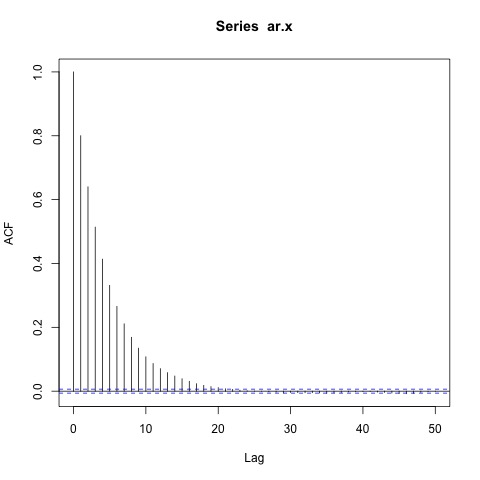
\includegraphics[width=5cm]{acf_ar.jpg}
        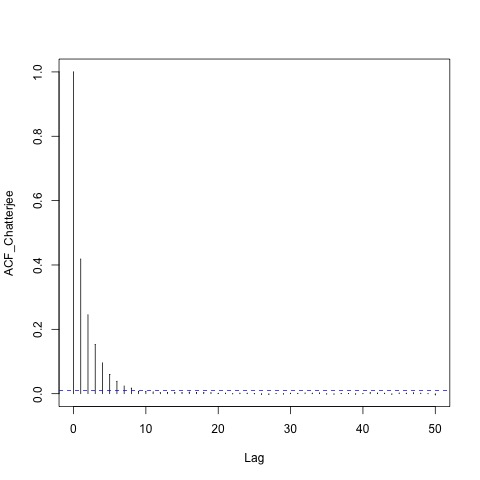
\includegraphics[width=5cm]{acf_ar_chatterjee.jpg}
\end{frame}

\begin{frame}
    \frametitle{Simulations}
    \begin{itemize}
        \item Metropolis-Hastings algorithm with initial distribution as Exp(0.01) and target distribution $\mathcal{N}(0, 1)$.
    \end{itemize}
    \vspace{2em}
    \centering
        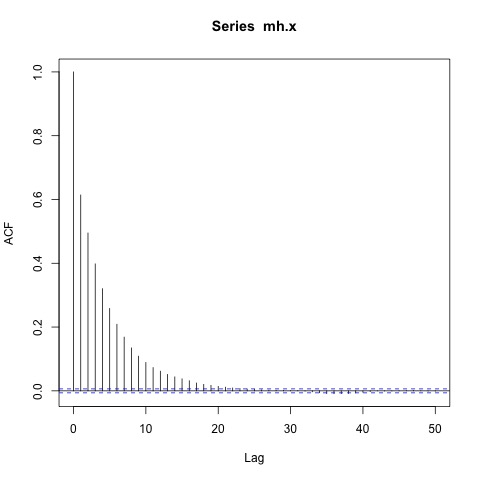
\includegraphics[width=5cm]{acf_mh.jpg}
        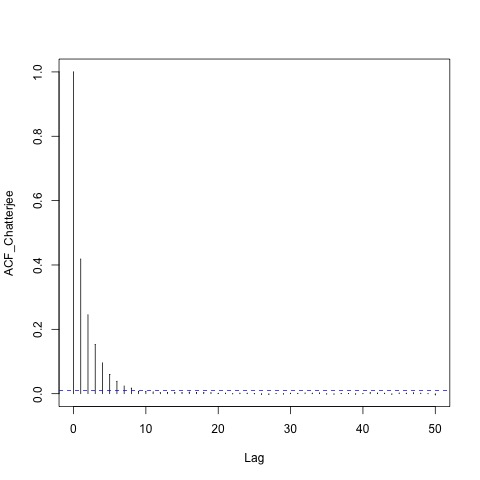
\includegraphics[width=5cm]{acf_mh_chatterjee.jpg}
\end{frame}

\begin{frame}
    \vspace{8em}
    \centering
    \begin{LARGE}
    Thank you
    \end{LARGE}

\end{frame}

% \begin{frame} [allowframebreaks]\frametitle{References}
%         \bibliographystyle{apalike}
%         \bibliography{bibfile}
% \end{frame}

\end{document}